\documentclass[12pt]{article}
\usepackage[utf8]{inputenc}
\usepackage{amsmath, amssymb}
\usepackage{tikz}
\usepackage{geometry}
\usepackage{graphicx}
\usepackage{xcolor}
\geometry{margin=1in}

\begin{document}
\section*{Problema a}
Sean tres cargas puntuales ubicadas en el plano $x$-$y$ y cuyos valores son:

\begin{itemize}
  \item $q_1 = +2\,\mu C$ ubicada en $\vec{r}_1 = (-1,\ 0)\,\text{m}$
  \item $q_2 = +2\,\mu C$ ubicada en $\vec{r}_2 = (1,\ 0)\,\text{m}$
  \item $q_3 = -2\,\mu C$ ubicada en $\vec{r}_3 = (0,\ \sqrt{3})\,\text{m}$
\end{itemize}

Si la posición del punto en el plano es $ \vec{r}_P = (0,\ \frac{\sqrt{3}}{3})\,\text{m}$ Responda las siguientes preguntas:

\begin{center}
\begin{tikzpicture}[scale=2]
  \coordinate (A) at (-1,0);
  \coordinate (B) at (1,0);
  \coordinate (C) at (0,1.732);
  \coordinate (P) at (0,0.577);

  \draw[->] (-1.5,0) -- (1.5,0) node[right] {$x$};
  \draw[->] (0,-0.5) -- (0,2.1) node[above] {$y$};

  \filldraw[red] (A) circle (1.5pt) node[below left] {$q_1$};
  \filldraw[red] (B) circle (1.5pt) node[below right] {$q_2$};
  \filldraw[blue] (C) circle (1.5pt) node[above] {$q_3$};

  \filldraw (P) circle (1pt) node[left] {$P$};

  \draw[dashed] (P) -- (A);
  \draw[dashed] (P) -- (B);
  \draw[dashed] (P) -- (C);
\end{tikzpicture}
\end{center}

\section*{Preguntas}

\begin{enumerate}
\item[a)] Dibuje el\'ectrico en el punto $P$ generado por cada carga.
  \item[b)] Determine el campo el\'ectrico generado por cada carga en el punto $P$.
  \item[c)] Calcule el campo el\'ectrico total en el punto $P$.
  \item[d)] Determine la fuerza que experimentar\'ia una carga de prueba $q_0 = +1\,\mu C$ colocada en el punto $P$.
  \item[e)] Determine qu\'e valor debe tener la carga $q_3$ para que el campo el\'ectrico total se anule en el punto $P$.
  \item[f)] Interprete el resultado anterior obtenido. Qu\'e papel juega la simetr\'ia en la anulaci\'on del campo?
\end{enumerate}

\newpage
\section*{Figura}

\subsection*{a)}
\textcolor{blue}{(1.3\ \mbox{pts por cada carga positiva})} \\
\textcolor{blue}{(1.4\ \mbox{pts por la carga negativa})}
\begin{center}
\includegraphics[width=0.55\textwidth]{campo1.png} % Aquí va la imagen generada externamente
\end{center}

\subsection*{b) Campo el\'ectrico generado por cada carga}

\textbf{Datos:} $k = 8.99 \times 10^9\,\text{Nm}^2/\text{C}^2$, $q = 2 \times 10^{-6}\,\text{C}$, $\vec{r}_P = (0,\ 0.577)$ \\
\textcolor{blue}{(1.3\ \mbox{pts})}
\textbf{Para $q_1$:}
\[\vec{r}_P - \vec{r}_1 = (1, 0.577),\quad |\vec{r}_P - \vec{r}_1|^3 \approx 1.539\]
\[\vec{E}_1 = \frac{8.99 \times 10^9 \cdot 2 \times 10^{-6}}{1.539} (1, 0.577) \approx 11\,688 (1, 0.577) = (11\,688, 6\,743)\,\text{N/C}\]
\textcolor{blue}{(1.3\ \mbox{pts})}
\textbf{Para $q_2$:}
\[\vec{r}_P - \vec{r}_2 = (-1, 0.577),\quad \vec{E}_2 \approx 11\,688 (-1, 0.577) = (-11\,688, 6\,743)\,\text{N/C}\] 
\textcolor{blue}{(1.4\ \mbox{pts})}
\textbf{Para $q_3$:}
\[\vec{r}_P - \vec{r}_3 = (0, -1.155),\quad \vec{E}_3 = \frac{8.99 \times 10^9 \cdot (-2) \times 10^{-6}}{1.539} (0, -1.155) \approx (0, 13\,486)\,\text{N/C}\]

\subsection*{c) Campo total}
\textcolor{blue}{(4\ \mbox{pts})}
\[\vec{E}_\text{total} = \vec{E}_1 + \vec{E}_2 + \vec{E}_3 = (0, 6\,743 + 6\,743 + 13\,486) = (0, 26\,972)\,\text{N/C}\]

\subsection*{d) Fuerza sobre $q_0 = +1\,\mu C$}
\textcolor{blue}{(4\ \mbox{pts})}
\[\vec{F} = q_0 \cdot \vec{E}_\text{total} = 10^{-6} \cdot (0, 26\,972) = (0, 0.027)\,\text{N}\]

\subsection*{e) Valor de $q_3$ para anular el campo en $P$}
\textcolor{blue}{(2\ \mbox{pts})}
\[\vec{E}_1 + \vec{E}_2 = (0, 13\,486) \Rightarrow \vec{E}_3 = (0, -13\,486)\] \\
\textcolor{blue}{(2\ \mbox{pts})}
\[q_3 = \frac{-13\,486 \cdot 1.539}{8.99 \times 10^9 \cdot 1.155} \approx -4.00 \times 10^{-6}\,\text{C} = -4.00\,\mu C\]


%\subsection*{f) Interpretaci\'on}
%La simetr\'ia del tri\'angulo hace que las componentes horizontales de los campos generados por $q_1$ y $q_2$ se cancelen. Las componentes verticales se suman y solo pueden anularse si la tercera carga genera un campo exactamente opuesto. Esa condici\'on ocurre s\'olo si $q_3 = -4.00\,\mu C$.

















\newpage

\section*{Problema b}


Sean tres cargas puntuales ubicadas sobre el eje $x$:

\begin{itemize}
  \item $q_1 = +3\,\mu C$ ubicada en $x_1 = -1\,\text{m}$
  \item $q_2 = -2\,\mu C$ ubicada en $x_2 = 1\,\text{m}$
  \item $q_3 = +1\,\mu C$ ubicada en $x_3 = 2\,\text{m}$
\end{itemize}

Considere la constante de Coulomb $k = 8.99 \times 10^9\,\text{Nm}^2/\text{C}^2$. Responda las siguientes preguntas:

\begin{center}
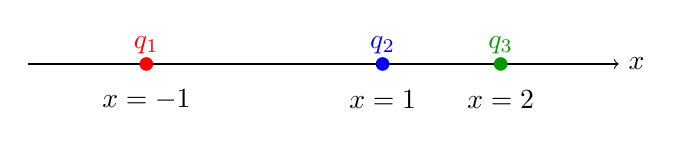
\begin{tikzpicture}[scale=1.5]
  \draw[->] (-2,0) -- (3,0) node[right] {$x$};
  \filldraw[red] (-1,0) circle (1.5pt) node[above] {$q_1$};
  \filldraw[blue] (1,0) circle (1.5pt) node[above] {$q_2$};
  \filldraw[green!60!black] (2,0) circle (1.5pt) node[above] {$q_3$};
  \node at (-1,-0.3) {$x = -1$};
  \node at (1,-0.3) {$x = 1$};
  \node at (2,-0.3) {$x = 2$};
\end{tikzpicture}
\end{center}

\begin{itemize}
   \item[a)] Dibuje el campo el\'ectrico generado por cada carga. 
     \item[b)] Calcule el campo el\'ectrico total en el punto $p = 3\,\text{m}$.
       \item[c)] Determine la fuerza que experimentar\'ia una carga de prueba $q_0 = +2\,\mu C$ colocada en el punto $p$.
  %\item[d)] Determine el valor de $x$ donde el campo el\'ectrico total es nulo cuando la carga $q_3$ ya no est\'a presente en el sistema.
	\item[d)] Determine la fuerza que experimentar\'ia una carga de prueba $q_0 = 1\,\mu C$ colocada en el punto $p$.
  \item[e)] Determine el valor de $x$ donde el campo el\'ectrico total es nulo cuando la carga $q_3$ ya no est\'a presente en el sistema (no considere las cargas de prueba utilizadas en c y d).

\end{itemize}
  
\newpage



\section*{Solución}


\begin{enumerate}
  \item[a)] Dibuje los vectores campo el\'ectrico generados por cada carga.
	
\textcolor{blue}{(1.3\ \mbox{pts por cada carga positiva})} \\
\textcolor{blue}{(1.4\ \mbox{pts por la carga negativa})}

\includegraphics[width=0.55\textwidth]{campo2.png} % Aquí va la imagen generada externamente


\item[b)] Calcule el campo el\'ectrico total en el punto $p = 3\,\text{m}$.

El campo total en $p = 3\,\text{m}$ se obtiene sumando los campos generados por cada carga.
 

  \begin{itemize}
  \item Posiciones relativas:
  \begin{align*}
  \vec{r}_p-\vec{r}_1 &= (3 - (-1))\hat{i} = 4\,(\hat{i})\text{m} \\ 
  \vec{r}_p-\vec{r}_2 &= (3 - 1)\hat{i} = 2\,(\hat{i})\text{m} \\ 
  \vec{r}_p-\vec{r}_3 &= (3 - 2)\hat{i} = 1\,(\hat{i})\text{m} 
  \end{align*}
\textcolor{blue}{(1\ \mbox{pto})}\\


  \item Cálculo del campo de cada carga:
  \begin{align*}
  \vec{E}_1 &= k\cdot q_1 \cdot \frac{\vec{r}_p-\vec{r}_1}{||\vec{r}_p-\vec{r}_1||^3} = 8.99 \times 10^9 \cdot 3 \times 10^{-6}\cdot \frac{4\,}{4^3}\hat{i} = \frac{26.97 \times 10^3}{16}\hat{i} = 1685.6(\hat{i})\,\text{N/C} \\
   \vec{E}_2 &= k\cdot q_2 \cdot \frac{\vec{r}_p-\vec{r}_2}{||\vec{r}_p-\vec{r}_2||^3} = -8.99 \times 10^9 \cdot 2 \times 10^{-6}\frac{2}{2^3}\hat{i} = -4495.0\,(\hat{i})\text{N/C}  \\
   \vec{E}_3 &= k\cdot q_3 \cdot \frac{\vec{r}_p-\vec{r}_3}{||\vec{r}_p-\vec{r}_3||^3} =8.99 \times 10^9 \cdot 1 \times 10^{-6} \frac{1}{1^3}\hat{i} = 8990.0\,(\hat{i} )\text{N/C}
  \end{align*}
\textcolor{blue}{(2\ \mbox{pts})} \\


  \item Campo total:
  \[
  \vec{E}_\text{total} = (1685.6 - 4495.0 + 8990.0)\,\hat{i} = 8180.6\,\text{N/C}
  \] \\
	\textcolor{blue}{(1\ \mbox{pto})}
  \end{itemize}

  \item[c)] Determine la fuerza que experimentar\'ia una carga de prueba $q_0 = +2\,\mu C$ colocada en el punto $p$. Sabemos que:

  \[ \vec{F} = q_0 \cdot \vec{E}_\text{total} \]
  \[ \vec{F} = (2 \times 10^{-6}) \cdot 8180.6 = 0.0164\,(\hat{i})\text{N} \]
	
		\textcolor{blue}{(4\ \mbox{pts})} \\

  \item[d)] Determine la fuerza que experimentar\'ia una carga de prueba $q_0 = +1\,\mu C$ colocada en el punto $p$. Sabemos que:
	
  \[ \vec{F} = q_0 \cdot \vec{E}_\text{total} \]
  \[ \vec{F} = (1 \times 10^{-6}) \cdot 8180.6 = 0.0082\,(\hat{i})\text{N} \] 

\textcolor{blue}{(4\ \mbox{pts})} \\

 \item[e)] Determine el valor de $x$ donde el campo el\'ectrico total es nulo cuando la carga $q_3$ ya no est\'a presente en el sistema. El sistema queda con $q_1 = +3\,\mu C$ en $x = -1$ y $q_2 = -2\,\mu C$ en $x = 1$. Buscamos el punto $x$ donde:
  \[ \vec{E}_1(x) + \vec{E}_2(x) = 0 \]
	
	\textcolor{blue}{(1\ \mbox{pto})} \\
  Para $x > 1$:
  \begin{align*}
  \vec{E}_1(x) &= \frac{k \cdot q_1}{(x + 1)^2} \cdot \hat{i} \\
  \vec{E}_2(x) &= \frac{k \cdot (-2)}{(x - 1)^2} \cdot \hat{i}
  \end{align*}
  Igualamos:
  \[ \frac{3}{(x + 1)^2} = \frac{2}{(x - 1)^2} \Rightarrow \left(\frac{x - 1}{x + 1}\right)^2 = \frac{2}{3} \Rightarrow \frac{x - 1}{x + 1} = \sqrt{\frac{2}{3}} \]
	
	\textcolor{blue}{(2\ \mbox{pts})} \\
	
  Despejando:
  \[ x - 1 = \sqrt{\frac{2}{3}}(x + 1) \Rightarrow x(1 - \sqrt{2/3}) = 1 + \sqrt{2/3} \Rightarrow x = \frac{1 + \sqrt{2/3}}{1 - \sqrt{2/3}} \]
  \[ x \approx 4.10\,\text{m} \]
	
	\textcolor{blue}{(1\ \mbox{pto})} \\

 % \item[e)] Interprete el resultado anterior.
  %La anulaci\'on del campo depende de un equilibrio entre el valor de la carga y el cuadrado de la distancia. Como $q_1$ es mayor, el punto de anulaci\'on debe ubicarse m\'as cerca de $q_2$ (la de menor magnitud), pero alejado de ambas.
\end{enumerate}






















\end{document}

